\subsection{Dateikonzept} \label{json_config_files}
Für das Dateikonzept wurden drei Dateitypen auf Basis von \acs{json} Dateien entwickelt. Abb. \ref{fig:vereinfachter_aufbau_dateikonzept} dient dem besseren Verständnis des Dateikonzepts. Hauptsächlich zeigt diese einen vereinfachten Aufbau der Komponenten, die von der Firma Bösch zur Entwicklung einer \acs{rltanzeige} bereitgestellt wurden, und die dazugehörigen Konfigurationsdateien. Die \acs{rltanzeige} selbst ist über den Bus mit einem Ventilator von ebm-papst sowie einem \gls{qbm}9711 von Siemens verbunden. Der Ventilator verfügt lediglich über integrierte Sensorik. Der \gls{qbm}9711 hingegen verfügt über zwei integrierte Luftdruck-Sensoren (interne Ports 1 und 2), zwei (an die Ports Analog Input 1 und 2) extern angeschlossene Temperatursensoren, eine (an den Port Analog Output 1) extern angeschlossene Klappe und ein (an den Port Analog Output 2) extern angeschlossenes Relais.


\begin{figure}[H]
	\centering
	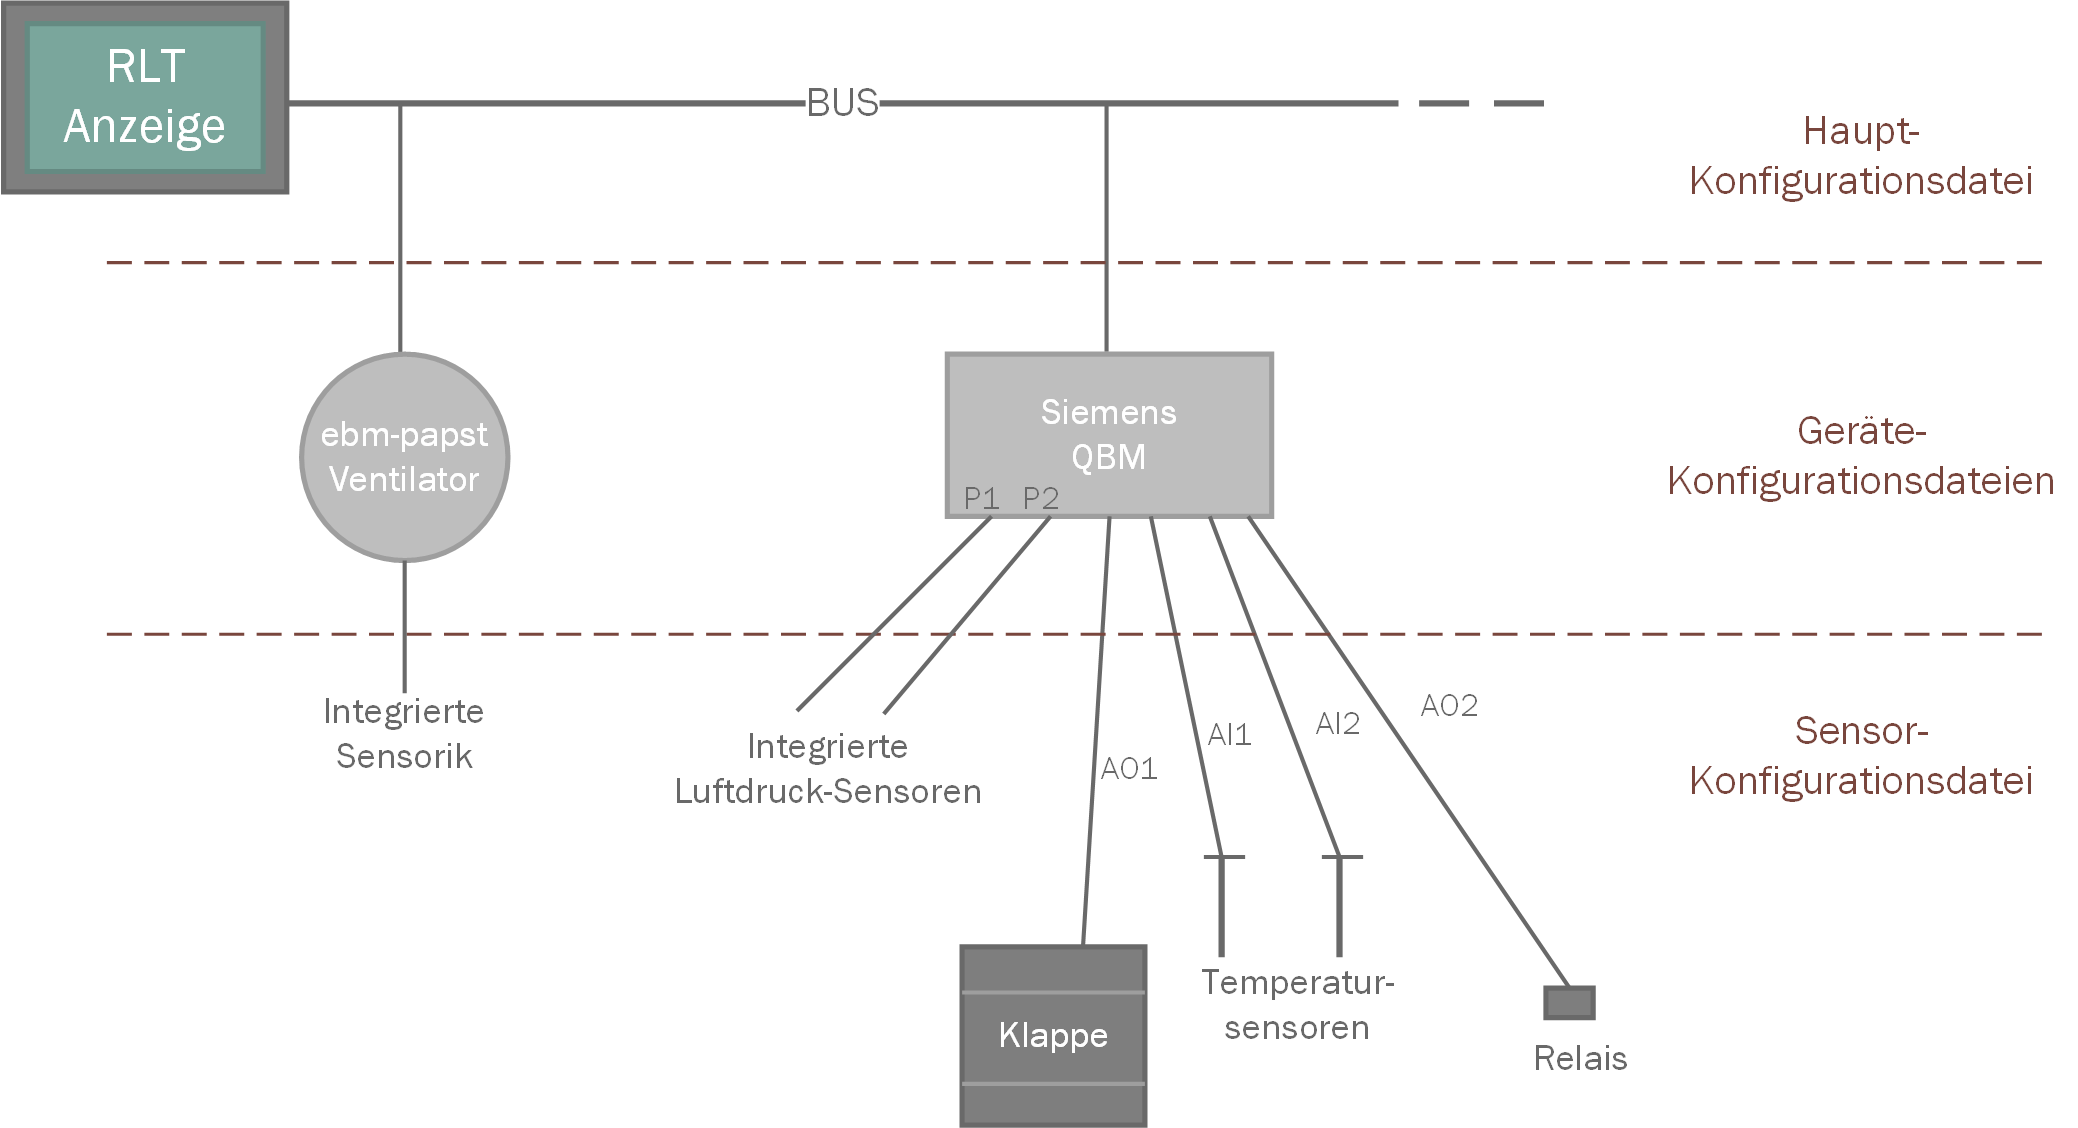
\includegraphics[width=\textwidth]{Komponenten_simpler_Aufbau_fuer_Dateikonzept}
	\caption{Vereinfachter Aufbau der Komponenten \label{fig:vereinfachter_aufbau_dateikonzept}}
\end{figure}

\newpage
Es folgt eine aufbauende Beschreibung und Erklärung der drei Dateitypen:
%Fenkart fragen, ob ich bei den Geräten auf seinen Teil verweisen kann
% Wer beschreibt baud_rate, register, adresse, function code \ref{modbus_funktionsweise}

\begin{enumerate}
	
	\item \textbf{Haupt-Konfigurationsdatei} (\enquote{main\_config\_file.json}):
	Wie in Kapitel \ref{gui_design} beschrieben, ist zur übersichtlichen Darstellung der Messwerte eine Aufteilung in mehrere Abschnitte bzw. Seiten erforderlich. Auf diesen Seiten werden jeweils sinngemäß Messwerte zusammengefasst. Die Konfiguration der Seiten erfolgt in der Haupt-Konfigurationsdatei mithilfe von zwei parallelen Arrays: dem \enquote{pages}-Array und dem \enquote{devices}-Array. 	
	
	Im \enquote{devices} Array werden alle Komponenten \bzw Quellen der \acs{rltanlage}, nämlich Ventilatoren und \gls{qbm}s (vgl. Abb. \ref{fig:vereinfachter_aufbau_dateikonzept}), aufgeführt, von denen Messwerte ausgelesen werden sollen. Die Parameter des \enquote{devices} Arrays sind in Tab. \ref{tab:devices_array_parameter} näher erläutert.

 \begin{longtable}{p{\dimexpr 0.15\textwidth-2\tabcolsep} p{0.52\textwidth} | p{0.28\textwidth}}
    \caption{Parameter des \enquote{devices} Array der Haupt-Konfigurationsdatei}
    \label{tab:devices_array_parameter}
    \\ \toprule
    \textbf{Name} & \textbf{Beschreibung} & \textbf{Beispiel}
    \\ \midrule
    \endfirsthead
    \caption{Parameter des \enquote{devices} Array der Haupt-Konfigurationsdatei (Fortsetzung)}
    %
    \\ \toprule
    \textbf{Name} & \textbf{Beschreibung} & \textbf{Beispiel}
    \\ \midrule
    \endhead
    %
    \midrule
    \multicolumn{3}{r}{{Fortsetzung auf der nächsten Seite}} 
    \\ \bottomrule
    \endfoot
    %
    \bottomrule
    \endlastfoot
    device     	& Angabe des Gerätetyps, indem auf den Namen der zugehörigen Geräte-Konfigurationsdatei referenziert wird. & 	
    \begin{jsonTable}
"device": "QBM97XX"
    \end{jsonTable}  
    \\
    id         	& Beliebig auswählbare, jedoch eindeutige Bezeichnung für das Gerät. Mit der \enquote{id} wird im \enquote{pages} Array auf das Gerät referenziert.  & 	
    \begin{jsonTable}
"id": "QBM1"
    \end{jsonTable}  
    \\
    baud\_rate	& Eingestellte Baudrate (vgl. Kapitel \ref{baud_rate}). Ist bei allen Komponenten einer \acs{rltanlage} gleich. & 	
    \begin{jsonTable}
"baud_rate": 19200
    \end{jsonTable}  
    \\
    mbaddress	& Die \gls{modbus} Adresse des Geräts. (vgl. Kapitel \ref{modbus_funktionsweise}) & 	
    \begin{jsonTable}
"mbaddress": 1
    \end{jsonTable}  
    \\
    parity	& Parität. Mögliche Werte: \enquote{even}, \enquote{odd} oder \enquote{none} (vgl. Kapitel \ref{modbus_uebertragungsarten}) & 	
    \begin{jsonTable}
"parity": "even"
    \end{jsonTable}  
    \\
    stop\_bits	& Anzahl der Stopbits einer Nachricht (vgl. Kapitel \ref{modbus_uebertragungsarten}) & 	
    \begin{jsonTable}
"stop_bits": 1
    \end{jsonTable}  
    \\
    zero\_based	& Gibt an, ob die \gls{modbus} Register von 0 oder 1 ausgehend gezählt werden. Mögliche Werte: \enquote{true} oder \enquote{false}.
    
    (Bemerkung: Bei Siemens \gls{qbm}s normalerweise \enquote{false}, bei ebm-papst Ventilatoren \enquote{true}) & 	
    \begin{jsonTable}
"zero_based": false
    \end{jsonTable}  
    \\
    sensors	& Array aller am Gerät angeschlossenen Sensoren. Bei Ventilatoren und Ausgabeports, deren Werte ausschließlich von Python Funktionen zur Weiterverarbeitung genutzt werden (Erklärung in Kapitel \ref{python_functions}), wird auf die Angabe verzichtet. 
    
    Die zwei Parameter, die für jedes Objekt dieses Arrays angegeben werden, sind in Tab. \ref{tab:sensors_array_parameter} zu finden. & 	
    \begin{jsonTable}
"sensors": [ ]
    \end{jsonTable}  
    \\
\end{longtable}
	
\begin{table}[H]
    \caption{Parameter des Unterarray \enquote{sensors}}
    \label{tab:sensors_array_parameter}
    \begin{tabular}{p{\dimexpr 0.12\textwidth-2\tabcolsep} p{0.53\textwidth} | p{0.3\textwidth}}
        \toprule
        \textbf{Name} & \textbf{Beschreibung} & \textbf{Beispiel} \\
        \midrule
        port   	& Verweist auf den Ausgabeport aus der Geräte-Konfigurationsdatei (siehe Tab. \ref{tab:ports_array_parameter}). Mögliche Werte können also \zB der Datei \enquote{QBM97XX.json} entnommen werden. & 	
        \begin{jsonTable}
"port": "AI1"
        \end{jsonTable}  
        \\
        type 	& Verweist auf einen Sensor aus der Sensor-Konfigurationsdatei. Mögliche Werte können also \zB der Datei \enquote{sensors.json} entnommen werden. & 	
        \begin{jsonTable}
"type": "LG-NI1000"
        \end{jsonTable}  
        \\
        \bottomrule
    \end{tabular}
\end{table}
					
\end{enumerate}



